\chapter{INN}

\section{Motivation}
\subsection{Background}

 Currently, when there is packet loss, signaled by duplicate ACKs (DUP ACKs), the DUP ACKs will traverse all the way back to the host (\textbf{Figure \ref{tradition-tcp}}). The host receives the DUP ACKs, then resends the packet. The goal of my project is to implement a fast TCP recovery mechanism, which aims to reduce the response time to DUP ACKs and reduce changes to the congestion window by retransmitting packets from within the network (e.g., from the switch), instead of sending the DUP ACKs back to the host (\textbf{Figure \ref{project-tcp}}). The implementation will be based on KVS concepts, where the key is the flow Id and sequence number, and the value is the packet.
 
For this project, I will be using the P4 programming language \cite{p4.org}. It is a language designed to allow the programming of packet forwarding planes. Besides, unlike general purpose languages such as C or Python, P4 is domain-specific with a number of constructs optimized around network data forwarding, hence is well suited to such a network application. 

\vspace*{5mm}

 \begin{figure}[h]
	\centering
	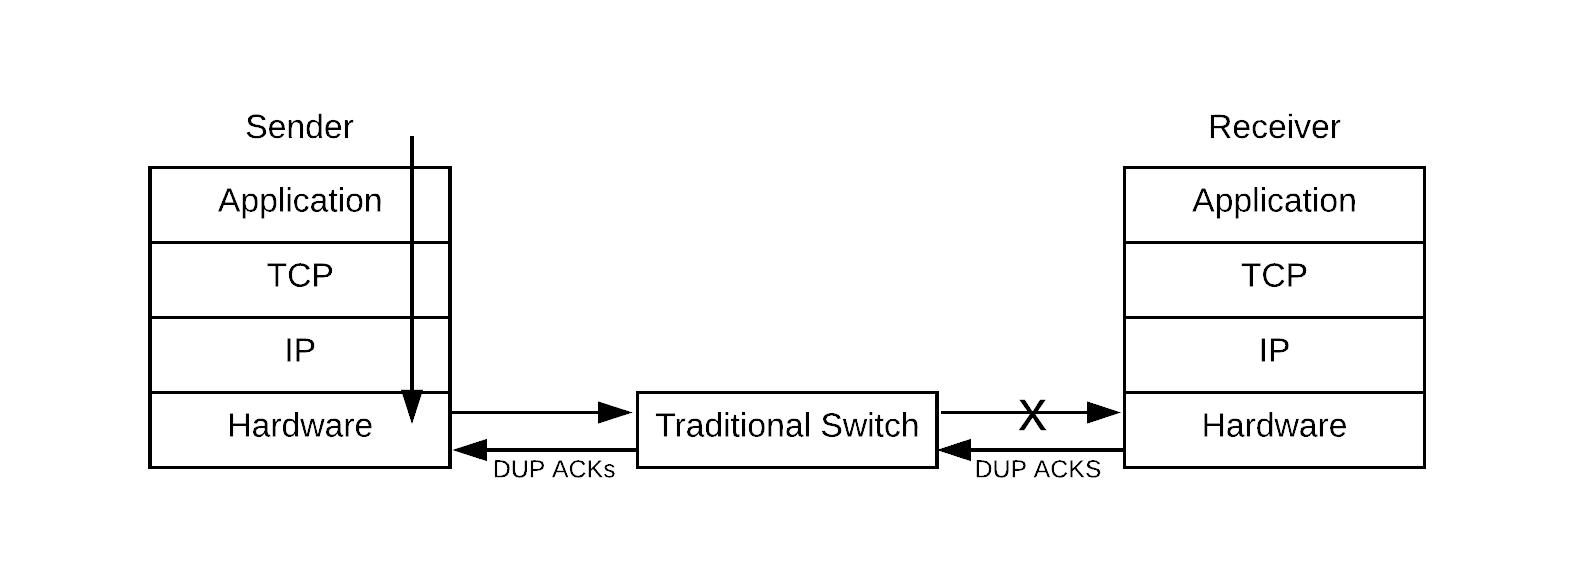
\includegraphics[width=\textwidth]{tradition-tcp.png}
	\caption{The standard convention of TCP handling.}
	\label{tradition-tcp}
\end{figure}

\begin{figure}[h]
	\centering
	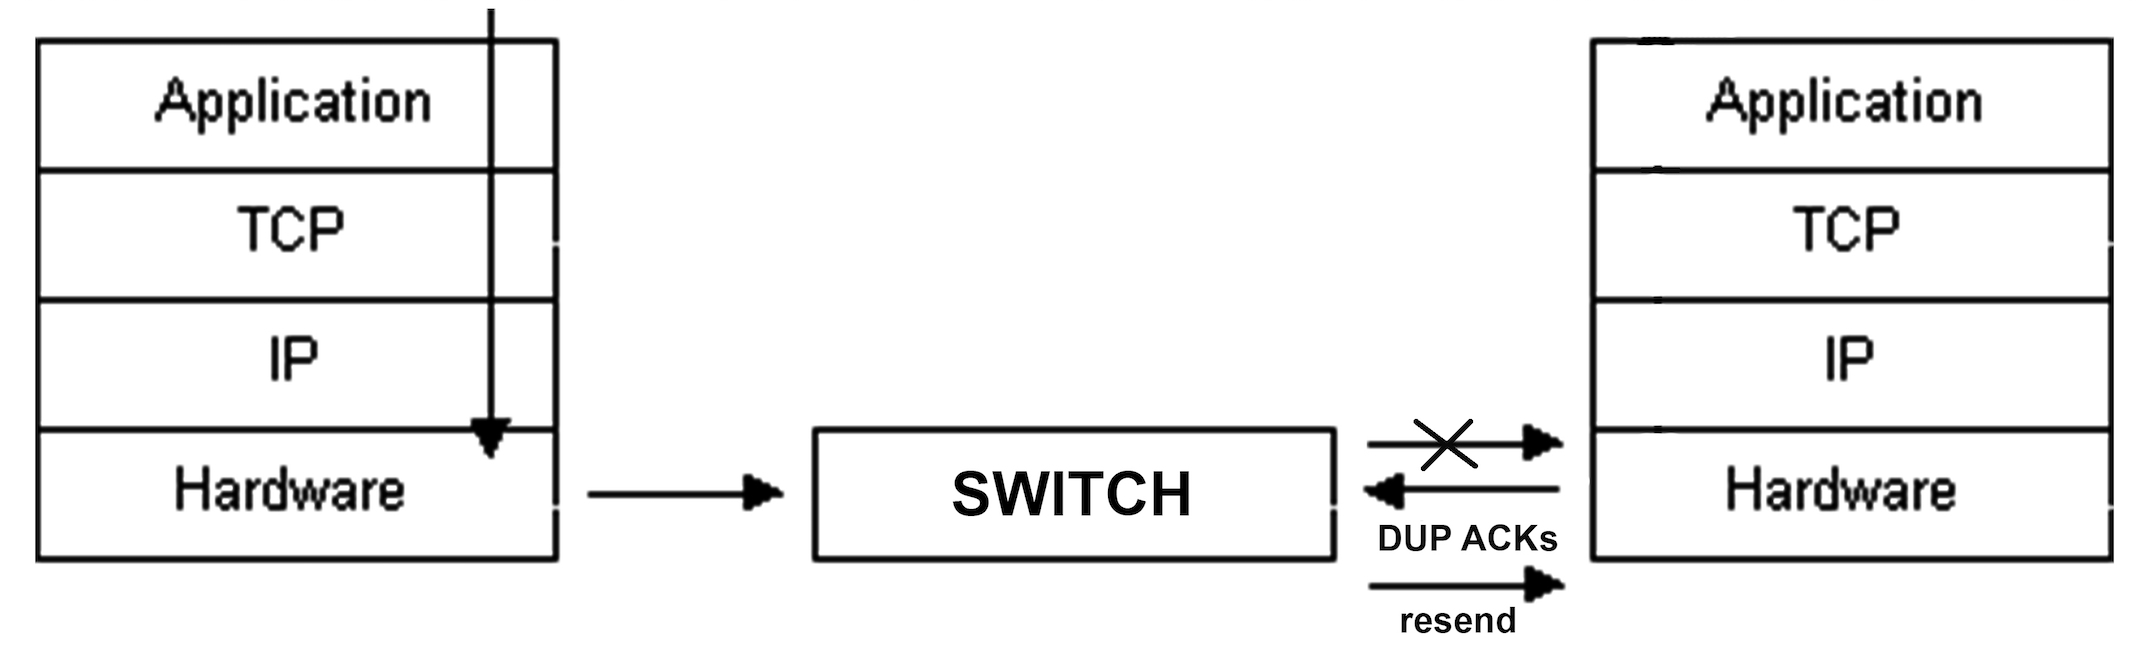
\includegraphics[width=\textwidth]{project-tcp.png}
	\caption{The proposed TCP handling.}
	\label{project-tcp}
\end{figure}


\section{Problem Outline}
\section{Related Work}
\newpage
Test